\documentclass{isprs}
\usepackage{subfigure}
\usepackage{setspace}
\usepackage{geometry} 
\geometry{a4paper, top=25mm, left=20mm, right=20mm, bottom=25mm, headsep=10mm, footskip=12mm} 
%\usepackage{isprs}
%\usepackage[perpage,para,symbol*]{footmisc}
%\renewcommand*{\thefootnote}{\fnsymbol{footnote}}

\usepackage{color}
\definecolor{gray}{gray}{0.4}

\usepackage[pdftex]{hyperref}
\hypersetup{
colorlinks=true,
linkcolor=black,
anchorcolor=black,
citecolor=black,
filecolor=black,
menucolor=black,
runcolor=black,
urlcolor=gray
}
%\urlstyle{same}
\usepackage{breakurl}
\usepackage[super]{nth}
\usepackage[inline]{enumitem}
\usepackage{moreenum}
\usepackage{booktabs}
\newcommand{\urlhttp}[1]{\href{http://#1}{\nolinkurl{#1}}}
\newcommand{\urlhttps}[1]{\href{https://#1}{\nolinkurl{#1}}}

\begin{document}

\title{Tangible Landscape: Cognitively grasping the flow of water}

\author{
 B. A. Harmon\textsuperscript{a}\thanks{Corresponding author}
 , A. Petrasova\textsuperscript{a}, V. Petras\textsuperscript{a}, H. Mitasova\textsuperscript{a}, R. K. Meentemeyer\textsuperscript{a}}

\address
{
	\textsuperscript{a }Center for Geospatial Analytics, North Carolina State University - (baharmon, akratoc, vpetras, hmitaso, rkmeente)@ncsu.edu\\
}

\commission{}{} %This field is optional.
\workinggroup{} %This field is optional.
\icwg{}   %This field is optional.
\ths{16 - Perceptual and cognitive experiments with imagery and 3D models}

\abstract
{
Complex spatial forms like topography can be challenging to understand, much less intentionally shape, given the heavy cognitive load of visualizing and manipulating 3D form. Spatiotemporal processes like the flow of water over a landscape are even more challenging to understand and intentionally direct as they are dependent upon their context and require the simulation of forces like gravity and momentum. This cognitive work can be offloaded onto computers through 3D geospatial modeling, analysis, and simulation.
Interacting with computers, however, can also be challenging, often requiring training and highly abstract thinking. Tangible computing -- an emerging paradigm of human-computer interaction in which data is physically manifested so that users can feel it and directly manipulate it -- aims to offload this added cognitive work onto the body. We have designed Tangible Landscape, a tangible interface powered by an open source geographic information system (GRASS GIS), so that users can naturally shape topography and interact with simulated processes with their hands in order to make observations, generate and test hypotheses, and make inferences about scientific phenomena in a rapid, iterative process. Conceptually Tangible Landscape couples a malleable physical model with a digital model of a landscape through a continuous cycle of 3D scanning, geospatial modeling, and projection. 
We ran a flow modeling experiment to test whether tangible interfaces like this can effectively enhance spatial performance by offloading cognitive processes onto computers and our bodies. We used hydrological simulations and statistics to quantitatively assess spatial performance. We found that Tangible Landscape enhanced 3D spatial performance and helped users understand water flow. 
}

\keywords{embodied cognition, spatial thinking, physical processes, water flow, hydrology, tangible user interfaces, user experiment, 3D}

\maketitle

\begin{figure*}[ht!]
\begin{center}
		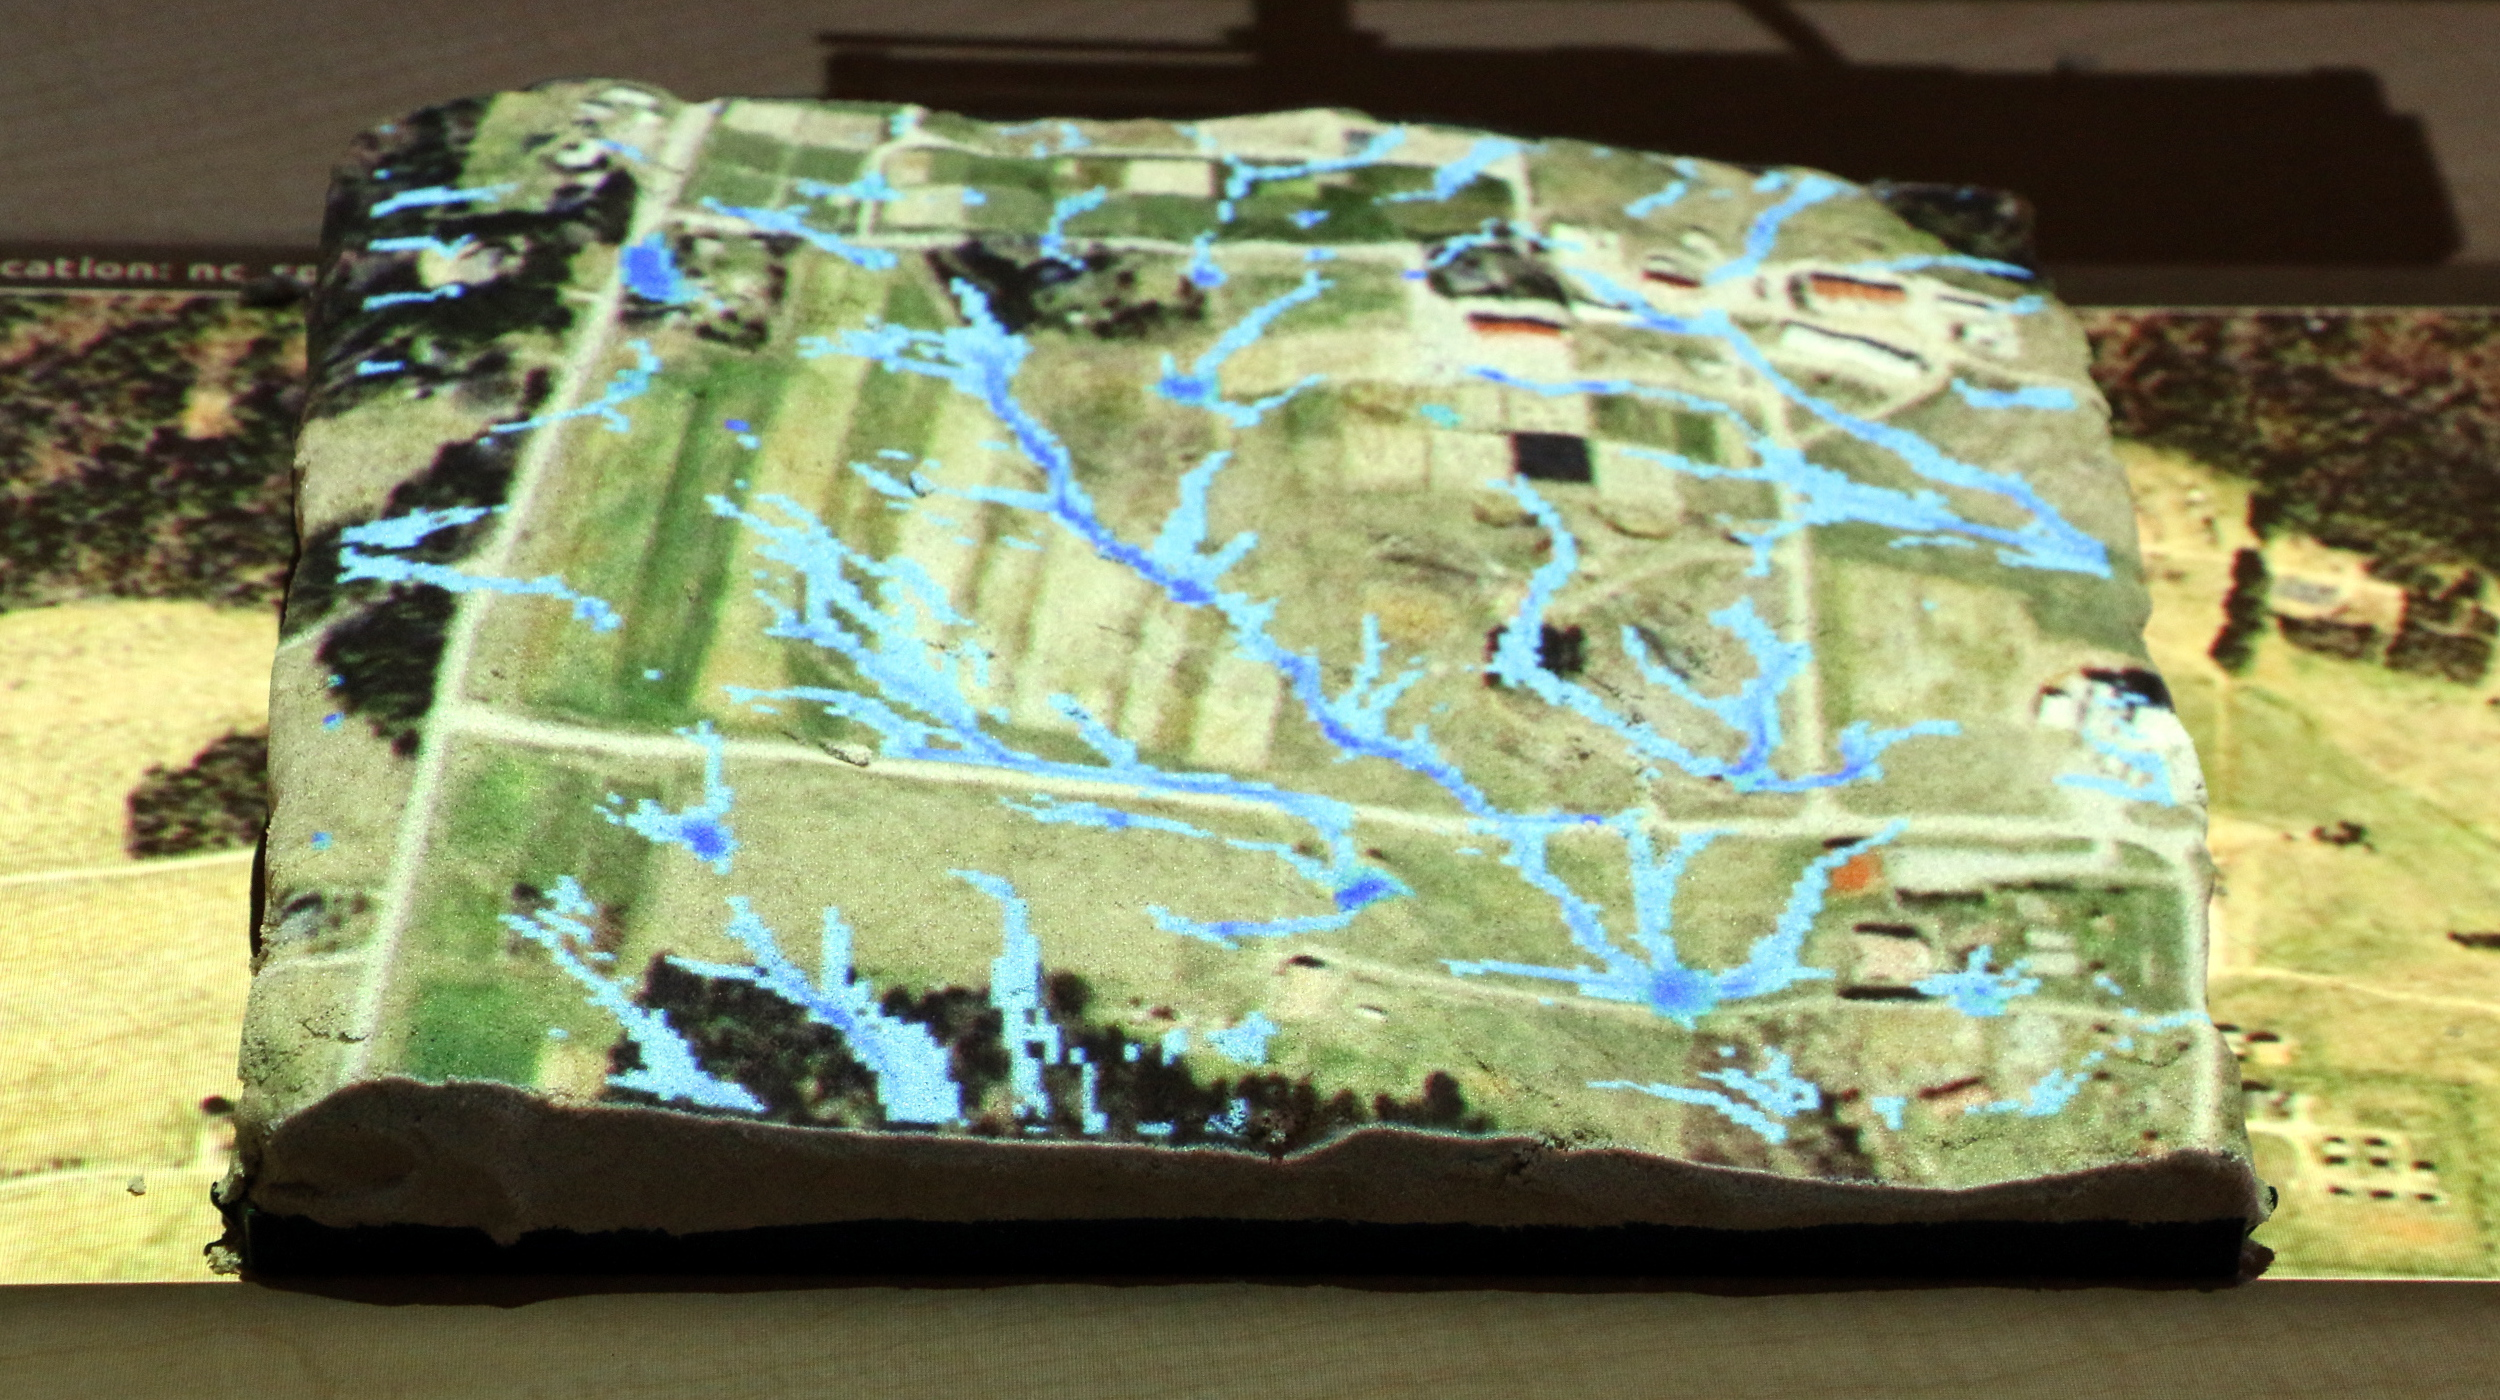
\includegraphics[width=0.33\textwidth]{figures/tl_sequence_1.jpg}
		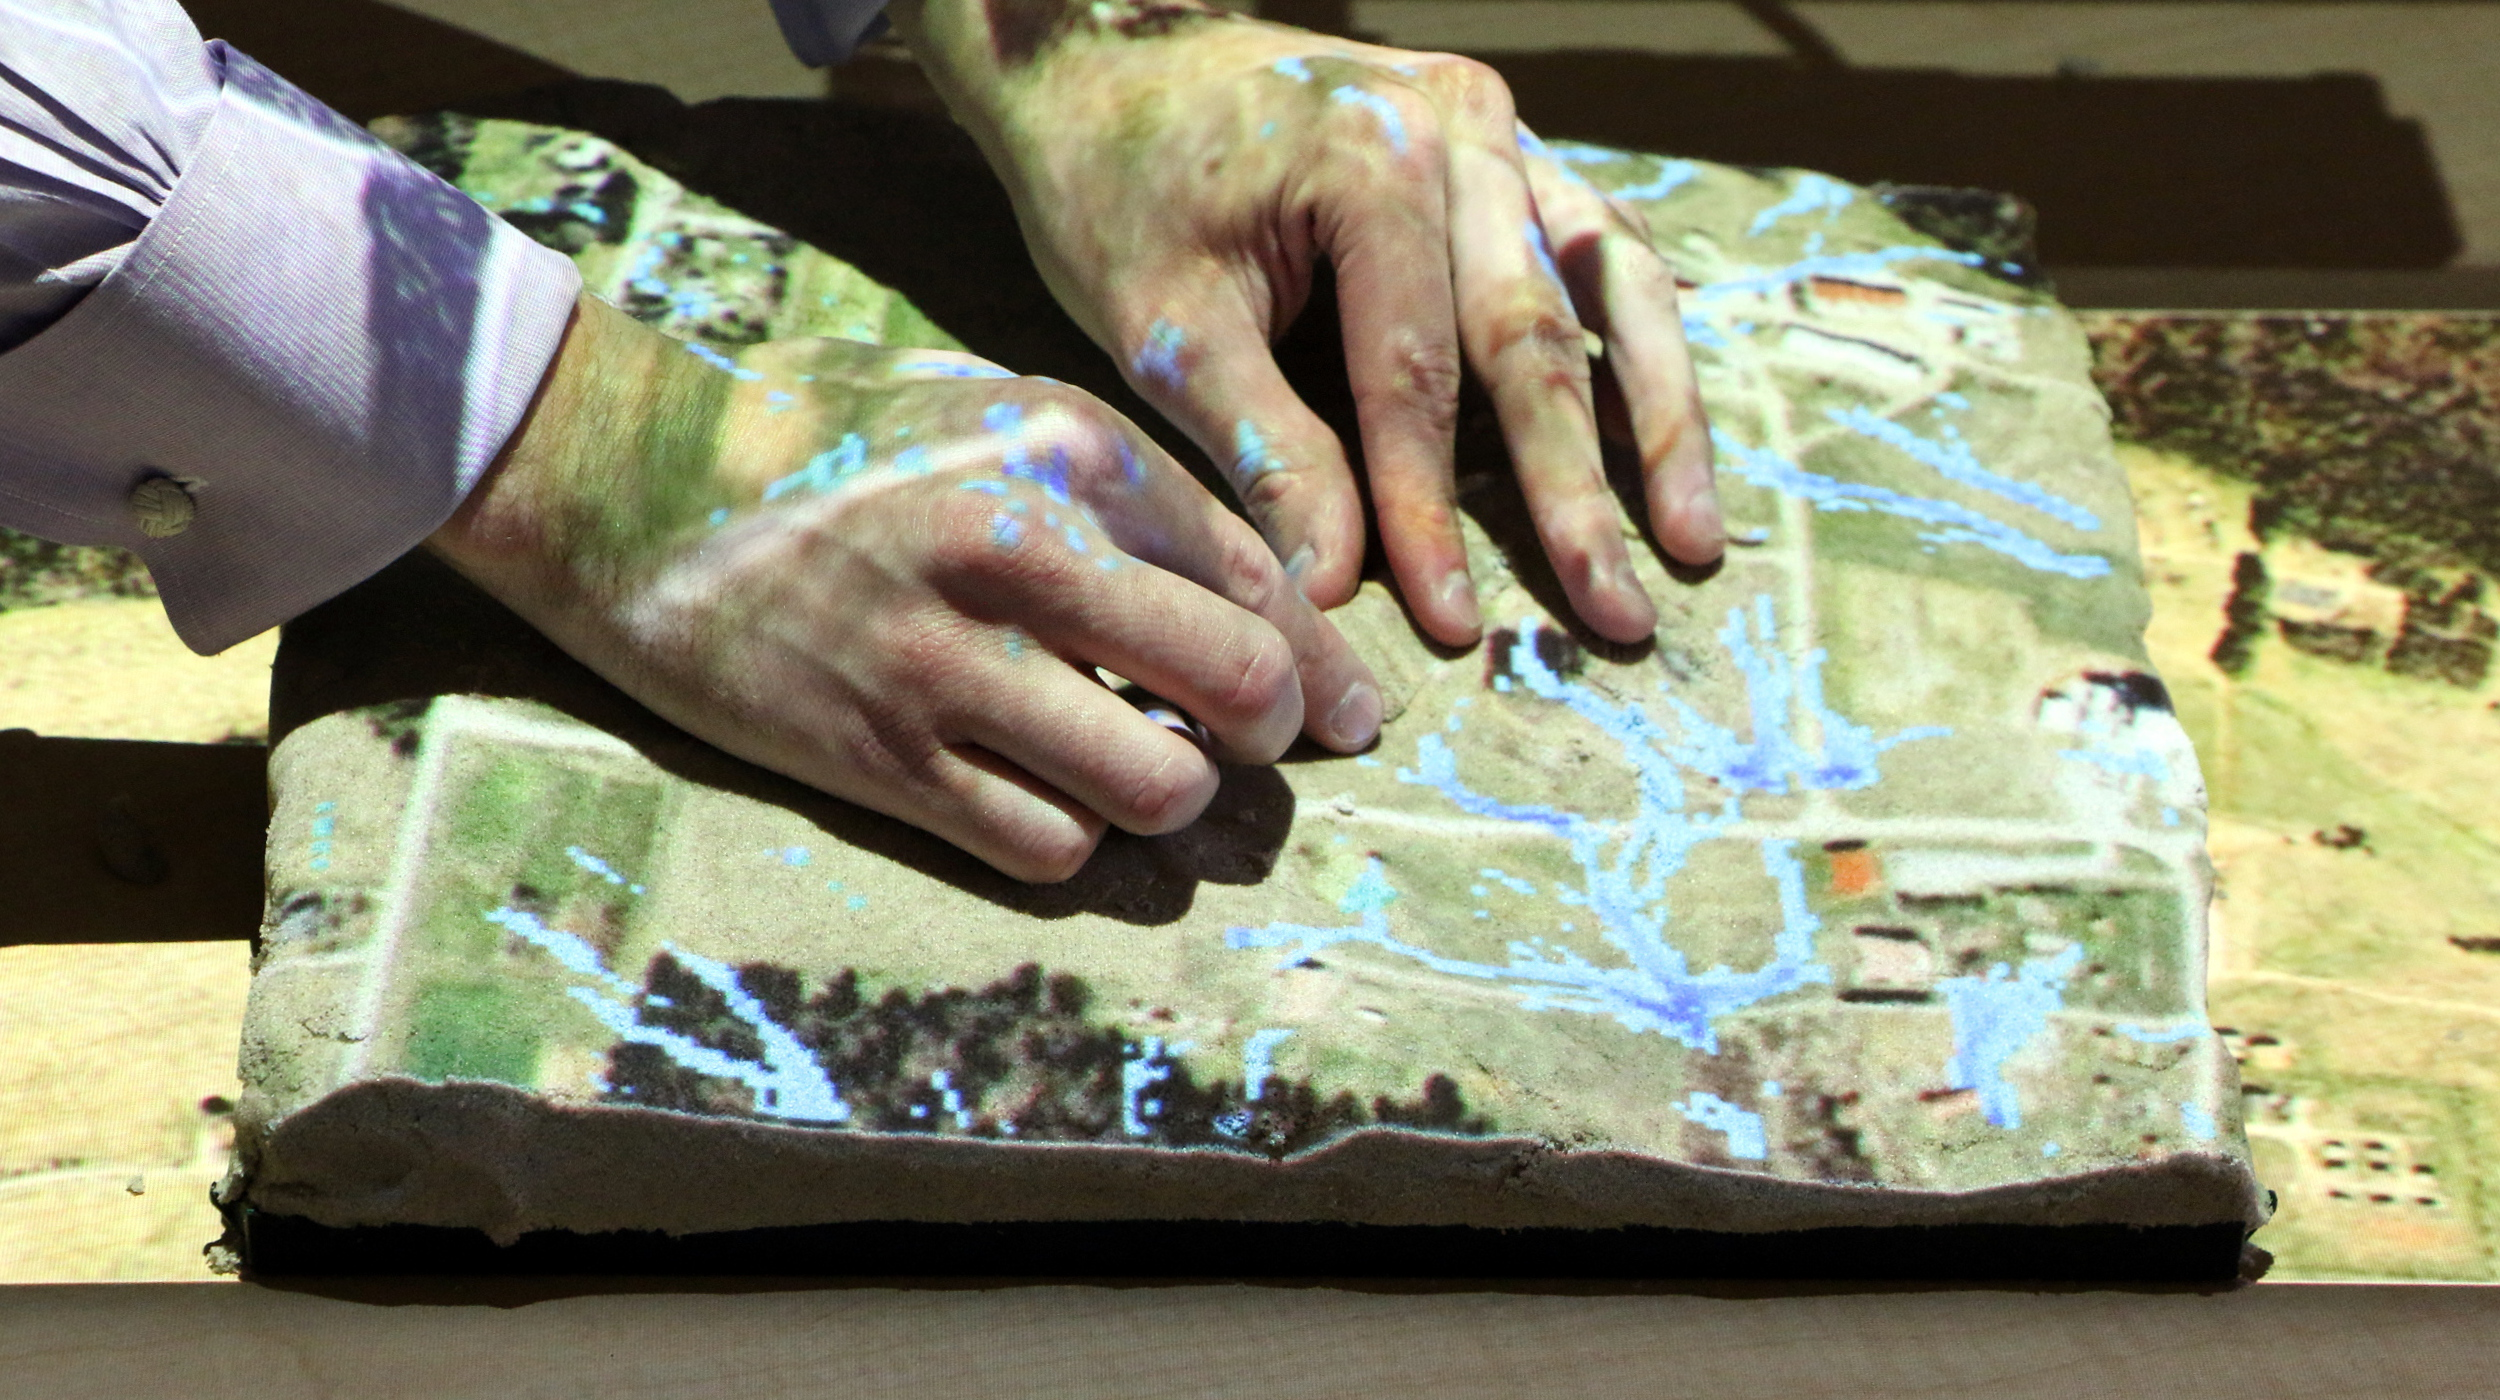
\includegraphics[width=0.33\textwidth]{figures/tl_sequence_2.jpg}
		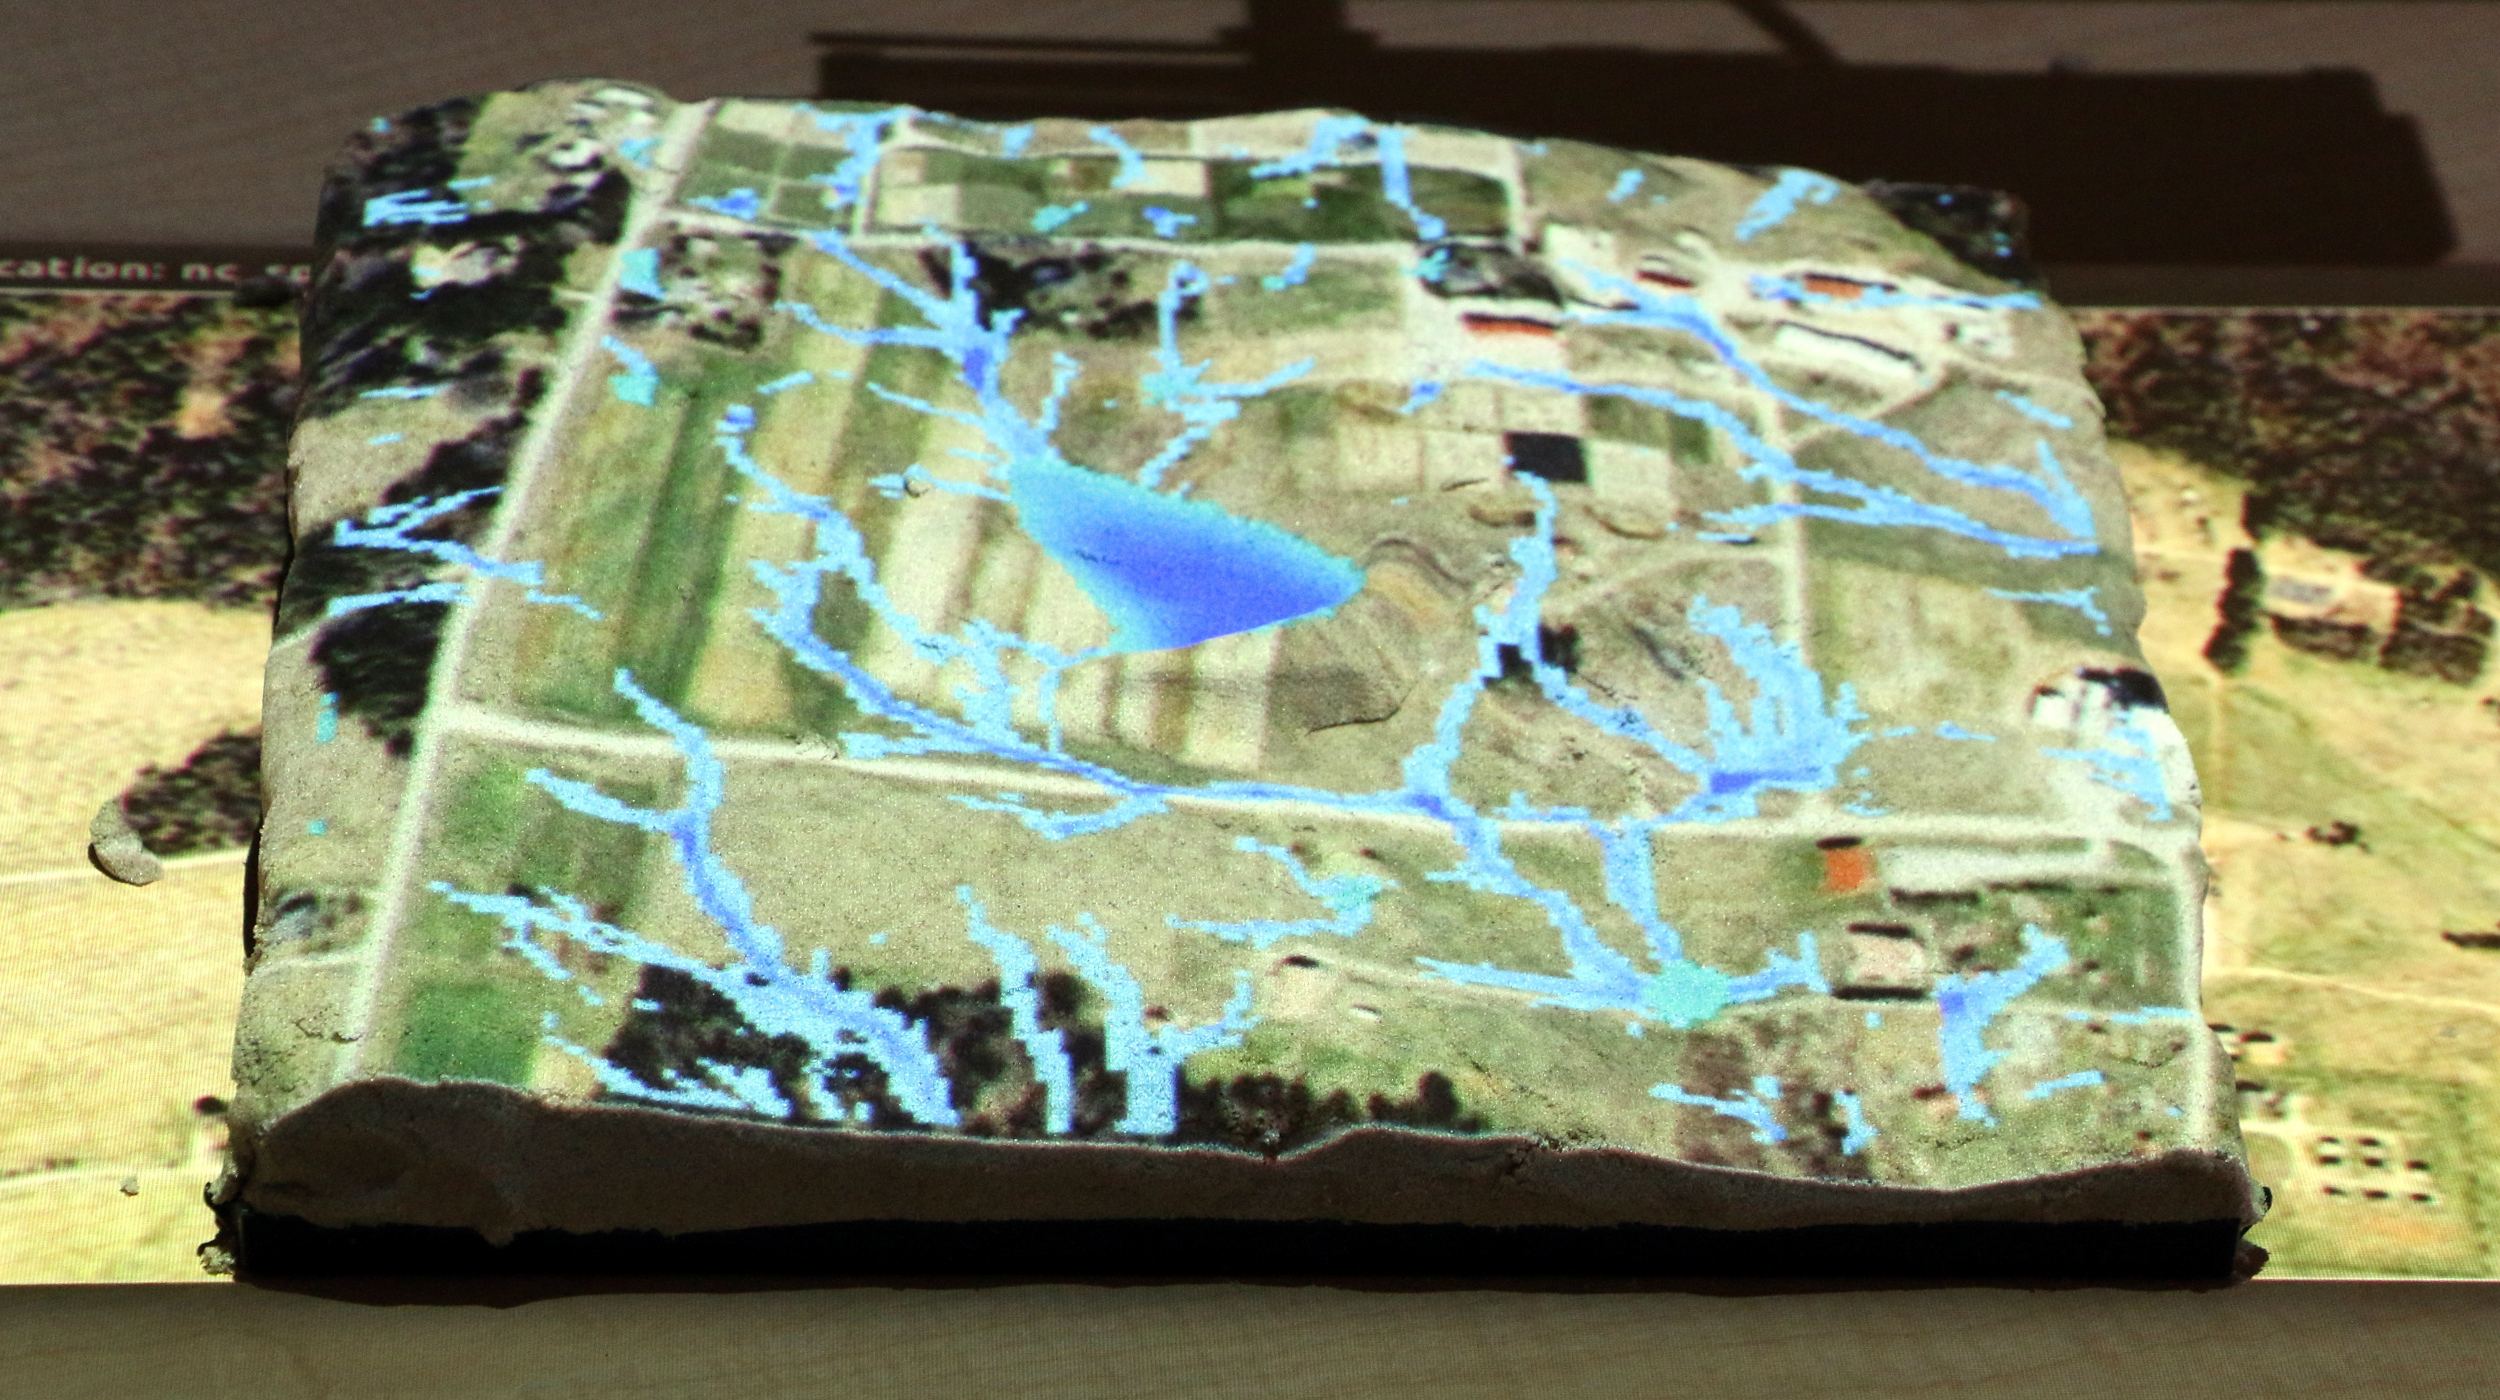
\includegraphics[width=0.33\textwidth]{figures/tl_sequence_3.jpg}
	\caption{Tangibly modeling the flow of water with Tangible Landscape}
	\label{fig:tl_flow}
\end{center}
\end{figure*}

\section{Introduction}\label{sec:introduction}

\subsection{Understanding physical processes}
% the challenges of understanding physical processes
Physical processes like the flow and dispersion of water are challenging to understand because they unfold in time and space, are controlled by their context, and are driven by forces like gravity and momentum. The flow of water across a landscape is controlled by the morphological shape and gradient of the topography. It is challenging to understand how water will flow across a landscape because one must not only understand how the shape and gradient of the terrain control the flow and dispersion of water locally, but also how water will flow between shapes and gradients -- how the morphology is topologically connected. Understanding a physical process requires thinking at and across multiple spatial scales simultaneously. 

% computational modeling in GIS
This cognitive work can be offloaded onto computers through 3D geospatial modeling, analysis, and simulation. Interacting with computers, however, can also be challenging requiring training and highly abstract thinking that adds a new cognitive burden.

\subsection{Tangible interfaces for GIS}
%
Tangible interfaces are designed to make interaction with computers easier and more natural
by physically manifesting digital data so that users can cognitively grasp it as an extension of their bodies, offloading cognition onto their bodies. 
%
In embodied cognition higher cognitive processes are built upon and grounded in sensorimotor processes -- upon bodily action, perception, and experience -- 
so thinking can performed subconsciously through action and extended with tools 
(such as pens and even computers) \cite{Kirsh2013}.
%
Tangible interfaces have been developed for geographic information systems (GIS) to ease the cognitive burden of complex spatial reasoning, spatial visualization, and human-computer interaction. 
%
Theoretically tangible interfaces for GIS should help users understand environmental processes
by giving multidimensional geospatial data an interactive, physical form 
that they can cognitively grasp and kinaesthetically explore in space and time. 

In a seminal paper Ishii and Ullmer envisioned tangible user interfaces that would 
`bridge the gap between cyberspace and the physical environment by making digital information (bits) tangible' \cite{Ishii1997}.
They described `tangible bits' as `the coupling of bits with graspable physical objects' \cite{Ishii1997}. 
Tangible interfaces like 
Urp \cite{Underkoffler1999}, Illuminating Clay \cite{Piper2002}, and SandScape \cite{Ratti2004} 
enriched physical models of urban spaces and landscapes with spatial analyses and simulations 
like wind direction, cast shadow, slope, aspect, curvature, and water direction
in order to enhance and streamline spatial thinking, design, and decision-making.

Many of the analyses used in Illuminating Clay were adapted from the open source GRASS GIS project \cite{Piper2002a} 
and eventually 
Illuminating Clay was coupled with GRASS GIS 
to draw on its extensive libraries for spatial computation. 
The aim of coupling Illuminating Clay with GRASS GIS was to 
`explore relationships that occur between different terrains, the physical parameters of terrains, and the landscape processes that occur in these terrains' \cite{Mitasova2006}. 
%
The effort to couple a physical landscape model with GRASS GIS led to the development of 
the Tangible Geospatial Modeling System \cite{Tateosian2010} and Tangible Landscape (Fig.~\ref{fig:tl_flow}) \cite{Petrasova2014,Petrasova2015}.

%% WHY
%While there are many reasons for developing tangible interfaces for GIS
%including intuitive form-finding, 
%streamlining analog and digital workflows, 
%and enabling multiple users to simultaneously interact in a natural way \cite{Ratti2004},
%the aim of this study is to...

\paragraph{Tangible Landscape}
Tangible Landscape -- a tangible user interface powered by GRASS GIS --
couples a physical and digital model of a landscape through a continuous cycle of 3D scanning, geospatial modeling, and projection
so that users can intuitively interact with the modeled landscape in near real-time 
(Fig.~\ref{fig:system_schema}). 
%
The physical model is often made of polymer-enriched sand so that users can easily sculpt forms in a medium that will hold its shape, has good plasticity, and has a familiar feel and aesthetic. 
% 
As users sculpt the physical model
the model is 3D scanned and
interpolated in GIS as a digital elevation model. 
The digital elevation model is used to compute 
geospatial analyses, models, and simulations, 
which are then projected back onto the physical model 
-- all in near real-time.
%
Conceptually, this enables users to hold a GIS in their hands -- 
feeling the shape of the earth, sculpting its topography, and directing the flow of water.
%
This should enable users to naturally model topography and interact with simulated physical processes in a rapid, iterative process 
of observation, hypothesis generation and testing, and inference. 

\begin{figure}[ht!]
\begin{center}
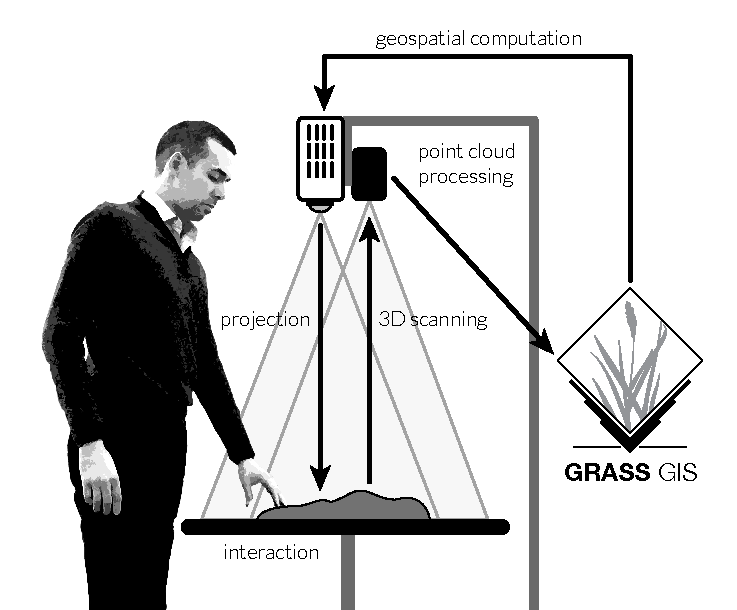
\includegraphics[width=1.0\columnwidth]{figures/system_schema_2.pdf}
\caption{How Tangible Landscape works: a near real-time feedback cycle of interaction, 3D scanning, point cloud processing, geospatial computation, and projection}
\label{fig:system_schema}
\end{center}
\end{figure}

\subsection{Cognitively grasping spatial processes}
The aim of this research was to study how tangible interfaces for GIS 
mediate spatial thinking about landscape processes like water flow. 
Theoretically a tangible interface for a GIS that enables intuitive digital sculpting while providing analytical %or simulated 
feedback should allow users to dynamically explore how topographic form influences landscape processes. 
With a physical model one can 
cognitively grasp topographic form, 
offloading the cognitive work of 
understanding and shaping topographic form onto the body. 
A GIS can offload the cognitive work of simulating complex physical processes
like the flow of water through computation. 
By combining these physical and computational affordances in a tangible interface for GIS we should be able to more easily understand and shape spatial processes. 
%In order to critique the theory of tangibles, identify cognitive challenges, and improve the design of tangibles...
We empirically tested how a tangible interface for GIS 
mediated spatial performance in a water flow modeling experiment. 

%This should be empirically tested in experiments and case studies so that we can critique and develop the theory grounding Tangible Landscape, identify cognitive challenges, and improve the design.  

\section{Methods}\label{sec:methods}
%
We conducted a terrain and water flow modeling experiment 
in which participants tried to recreate a given landscape. 
%
We quantitatively assessed their spatial performance using hydrological simulation, summary statistics, and cell-by-cell statistics.
%and qualitatively assessed their modeling process through observation and semi-structured interviews. 

\subsection{Flow modeling experiment}
%
In the experiment 11 participants were asked to sculpt a given landscape using different technologies -- 
first using Vue, a triangulated irregular network based 3D modeling program designed for intuitive terrain sculpting, 
and then using Tangible Landscape. 
%
The participants were asked to model a real landscape --
a region of Lake Raleigh Woods 
in Raleigh, North Carolina  -- 
%from a flat surface 
using each technology. 
%We used a real landscape because 
%computer generated landscapes look surreal, may lack distinct landforms, and may not form clear stream channels. 
We selected a region of the landscape with distinctive, 
clearly defined landforms -- a central ridge flanked by two stream valleys 
(see Fig.~\ref{fig:study_area}). 
The digital elevation model (DEM) for this region was interpolated from a 2013 airborne lidar survey using the regularized spline with tension method.

%\begin{enumerate*}[label=\raisenth*] 
%\item ...
%\end{enumerate*}

In the \nth{1} exercise 
each participant had 10 minutes to digitally sculpt the topography of the study landscape in Vue's terrain editor
using a physical model as a reference (see Fig.~\ref{fig:exercises}a).
%(Figure~\ref{fig:exercise_7}).
Participants were given a 2 minute introduction to terrain sculpting in Vue and then 10 minutes to experiment and become familiar with the interface before beginning the exercise. Vue's terrain editor was designed to emulate sculpting by hand -- there are tool brushes that are analogous to basic actions in sculpture including pushing, pulling, and smoothing. 

In the \nth{2} exercise each participant had ten minutes to  
sculpt the study landscape in polymeric sand
using Tangible Landscape's water flow simulation
%over the scanned landscape
as a guide (see Fig.~\ref{fig:exercises}b). 
%
As participants sculpted they could switch between projected maps of either the
\begin{enumerate*}[label=\alph*),font=\itshape]
\item simulated water flow across the given landscape that they were trying to replicate
\item or the simulated water flow across the scanned landscape.
\end{enumerate*}

\begin{figure}[ht!]
\begin{center}
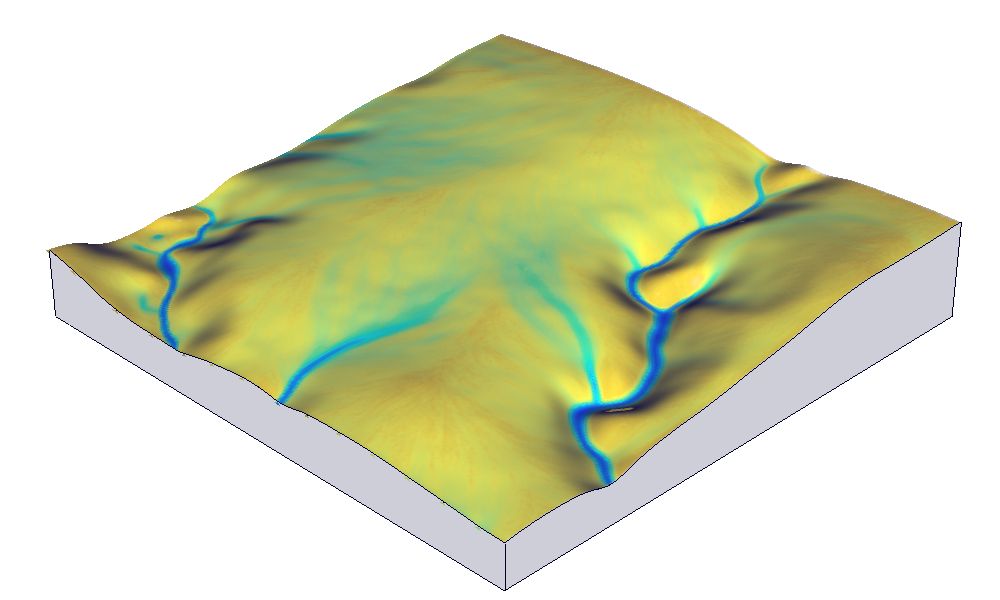
\includegraphics[width=1.0\columnwidth]{figures/depth_3d.png}
\caption{Our reference landscape with simulated water flow}
\label{fig:study_area}
\end{center}
\end{figure}

\begin{figure*}
\begin{center}
\subfigure[]{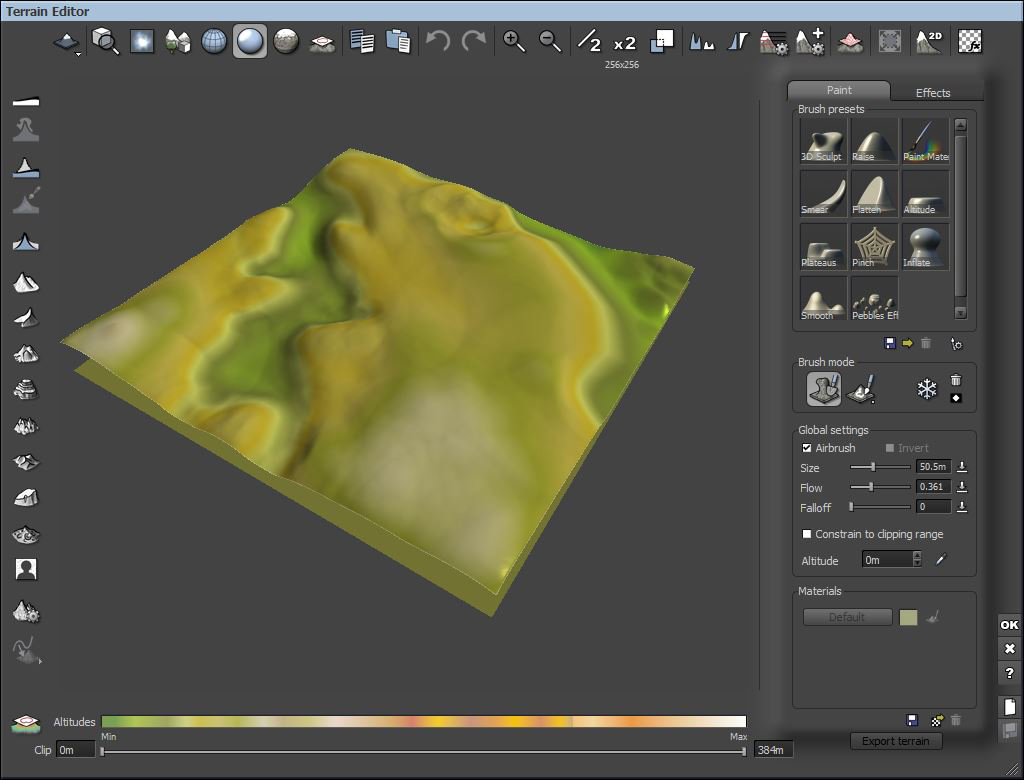
\includegraphics[height=150px]{figures/vue.jpg}}\hspace{1em}%
\subfigure[]{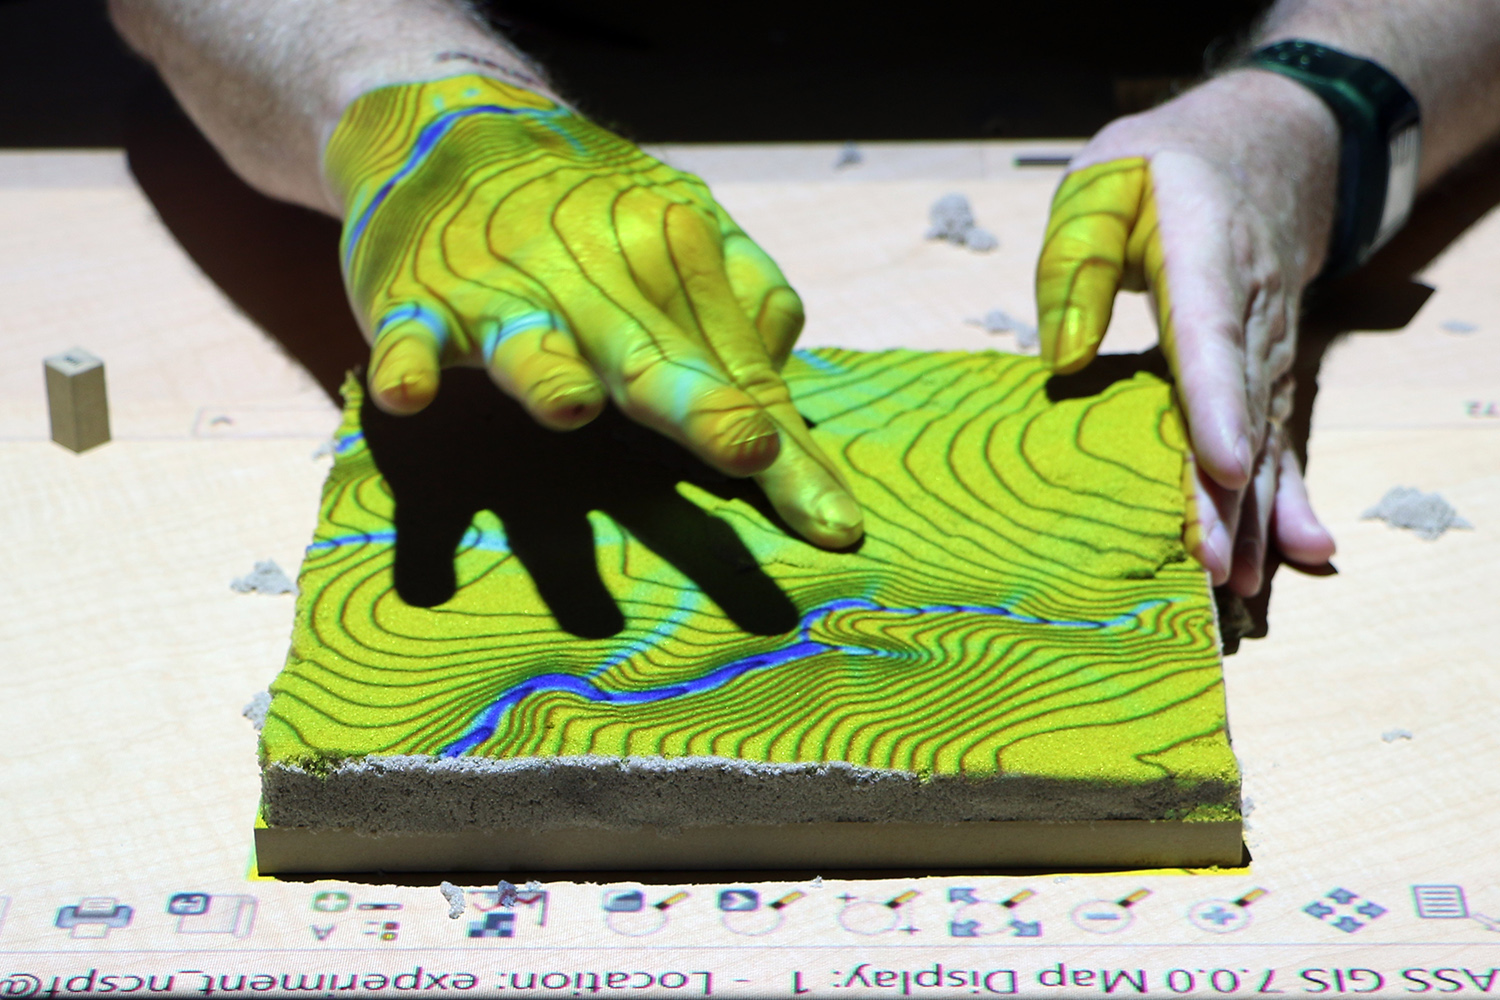
\includegraphics[height=150px]{figures/tl_water.jpg}}
\caption{(a) Digitally sculpting with Vue in the \nth{1} exercise and (b) tangibly sculpting with Tangible Landscape in the \nth{2} exercise}
\label{fig:exercises}
\end{center}
\end{figure*}

\subsection{Implementation}
% grass
We used GRASS GIS both
for geospatial computation with Tangible Landscape
and for the analysis of the results of the experiment.
% open source
The algorithms used in GRASS GIS are 
based on peer-reviewed scientific publications 
and have been 
transparently implemented 
with free, publicly available, version controlled source code. 
Open, transparent algorithms are needed to fully reproduce computational science \cite{Rocchini2012}. 
% simwe
In this experiment we used
the overland flow hydrologic simulation using a path sampling method (SIMWE) 
implemented in GRASS GIS as the module r.sim.water.

\paragraph{Shallow overland flow}
We simulated shallow overland water flow controlled by spatially variable topography, soil, landcover, and rainfall parameters using the SIMWE model to solve the continuity and momentum equations for steady state water flow with a path sampling method. 
%
Shallow water flow can be approximated by
the bivariate form of the St Venant equation:

\begin{equation}
\label{eq:water}
{\partial h({\bf r},t) \over \partial t} =
 i_e({\bf r},t) - \nabla \cdot {\bf q}({\bf r},t)
\end{equation}

where:

\hspace*{1em} ${\bf r}(x,y)$ is the position [m]

\hspace*{1em} $t$ is the time [s]

\hspace*{1em} $h({\bf r},t)$ is the depth of overland flow [m]

\hspace*{1em} $i_e({\bf r},t)$ is the rainfall excess [m/s]\\
\hspace*{1em} (rainfall $-$ infiltration $-$ vegetation intercept) 

\hspace*{1em} ${\bf q}({\bf r},t)$ is the water flow per unit width [$\rm m^2/s$].

%  diffusion wave approximation
By integrating a diffusion term $ \propto \nabla^2 [h^{5/3}({\bf r})]$ 
into
the solution of the continuity and momentum equations for steady state water flow
diffusive wave effects can be approximated
so that water can flow through depressions. 
%
\begin{equation}
\label{eq:difwater}
-{\varepsilon({\bf r})\over 2 }\nabla^2 [h^{5/3}({\bf r})]
+\nabla \cdot [ h({\bf r}){\bf v}({\bf r})] = i_e({\bf r})
\end{equation}

 where:
 
 \hspace*{1em} $\varepsilon({\bf r})$ is a spatially variable diffusion coefficient.

This equation is solved using a Green's function Monte Carlo path sampling method \cite{Mitasova2004}.

\subsection{Data collection and analysis}
%\paragraph{Quantitative}
We used summary and cell-by-cell statistics to compare the results of each exercise 
using the reference landscape as a baseline. 
The digital models sculpted in the \nth{1} exercise were manually georeferenced and imported into GRASS GIS as point clouds for modeling and analysis. 
The final state of the physical models sculpted in \nth{2} exercise were automatically 3D scanned, georeferenced, and imported into GRASS GIS as points clouds 
with Tangible Landscape for modeling and analysis. 
All of the point clouds were randomly resampled and interpolated as DEMs using the regularized spline with tension interpolation method \cite{Mitasova2005}. 
For each model we simulated shallow overland water flow, identified depressions,
and computed the difference between the modeled and reference water flow depth. 
To compute the difference we subtracted the modeled values from the initial, reference values. %(difference $=$ before $-$ after). 
We identified and computed the depth of depressions by generating a depressionless DEM and then calculating the difference between the DEM from the depressionless DEM.
%subtracting the DEM from the depressionless DEM.
Then we computed the mean, sum, and maximum of the water depths, the depressions, and the difference in water depths for each exercise in the experiment. 
We visually assessed the spatial pattern of water flow and continuity using these maps. 
%
In order to quantitatively compare how well the modeled streams matched the reference stream
we computed the distance between cells with concentrated water flow in the reference depth map and mean of the modeled depth maps. First we extracted points for each cell with high water depth values ($>=0.05$ ft) in the reference water depth raster and the mean water depth raster for each exercise. Then we calculated the minimum distance between the reference points and the nearest points from each exercise. 
%
In order to quantitatively compare the continuity of flow we computed the percentage of cells with depressions for each exercise.

%\paragraph{Qualitative}
%Participants' modeling processes
%were observed and documented during the experiment 
%with videos, photographs, and notes. 
%Semi-structured interviews were conducted with select participants
%after the experiment. 
%The interviews focused on 
%the intuitiveness and affordances of each technology, 
%participants' strategies and modes of representation, 
%their understanding of space in a given medium,
%and their spatial thought processes. 

\subsection{Code and data}

As a work of open science we invite you to
replicate or build upon this experiment by 
using or adapting our tangible interface, experimental methodology, code, and data. 
%
The python scripts for data processing and analysis used in this experiment 
are available on GitHub at 
\urlhttps{https://github.com/baharmon/tangible-water-flow}
released under the GNU General Public License (GPL). 
%
See the documentation in the GitHub repository for detailed instructions for replicating this experiment. 
%
The data used in this experiment are available on the Open Science Framework at \url{osf.io/zv3t6} under the Creative Commons Zero license.

GRASS GIS is available at
\urlhttps{https://grass.osgeo.org/} 
under the GNU GPL. 
%
Tangible Landscape is available at
\urlhttps{https://github.com/ncsu-osgeorel/grass-tangible-landscape} \\
under the GNU GPL. 
%
To build your own Tangible Landscape
see the documentation in the GitHub repository 
and refer to the book Tangible Modeling with Open Source GIS \cite{Petrasova2015}.

While the rest of the software used in this research is free and open source, 
Vue \footnote{\urlhttp{http://www.e-onsoftware.com/products/vue/}} is proprietary software. 
We used Vue's terrain editor for this study because it was designed specifically for intuitive terrain modeling, but 
open source 3D modeling programs like Blender \footnote{\urlhttps{https://www.blender.org/}} could be substituted for Vue. 
%

\section{Results}\label{sec:results}
%
The models sculpted with Tangible Landscape more accurately replicated the flow of water over the study landscape. 
%
The digitally sculpted models tended to have 
more diffuse water flow
and more water pooling in depressions, whereas 
%
the tangibly sculpted models tended to have 
more concentrated flow in stream channels
and less pooling in depressions.
%
Furthermore, 
the spatial distribution of water flow on the tangibly sculpted models 
more closely fit the distribution of water flow on the reference landscape. 

% water depth table
\begin{table}[h!]
\centering
\begin{tabular}{c c c c}
\toprule
Exercise & Mean & Max & Sum\\
\midrule
Reference & 0.48 & 0.01 & 786.25\\
Digital & 0.21 & 1.83 & 3.60\\
Tangible & 0.27 & 2.31 & 4.60\\ 
\bottomrule
\end{tabular}
\vspace*{0.5em}
\caption{Highest mean, maximum, and summed water depths (ft)}
\label{table:water_depth} 
\end{table}

% difference / distance
\begin{table}[h!]
\centering
\begin{tabular}{c c c}
\toprule
Exercise & Mean & Sum\\
\midrule
Digital & 21.13 & 29244\\
Tangible & 18.59 & 25724\\ 
\bottomrule
\end{tabular}
\vspace*{0.5em}
\caption{The minimum distances from reference stream cells to the nearest modeled cell with concentrated flow (ft)} 
%\caption{The mean and sum of the minimum distance  from cells with concentrated flow in the reference water depth to cells with concentrated flow in the mean water depth for each experiment (ft)} 
\label{table:distance} 
\end{table}

% depressions table
\begin{table}[h!]
\centering
\begin{tabular}{c c c}
\toprule
Exercise & Max & Sum \\
\midrule
Reference & 0.10 & 0.62\\
Digital & 24.5 & 53\\
Tangible & 22.2 & 44\\ 
\bottomrule
\end{tabular}
\vspace*{0.5em}
\caption{Highest max and summed depth of depressions (ft)}
\label{table:depressions} 
\end{table}

% cells with depressions table
\begin{table}[h!]
\centering
\begin{tabular}{c c}
\toprule
Exercise & Cells\\
\midrule
Reference & 0.00\%\\
Digital & 44.00\%\\
Tangible & 17.66\%\\ 
\bottomrule
\end{tabular}
\vspace*{0.5em}
\caption{Percent of cells with depressions (3 ft \textsuperscript{2})} 
\label{table:cells} 
\end{table}

%% difference / distance plot
%\begin{figure}[ht!]
%\begin{center}
%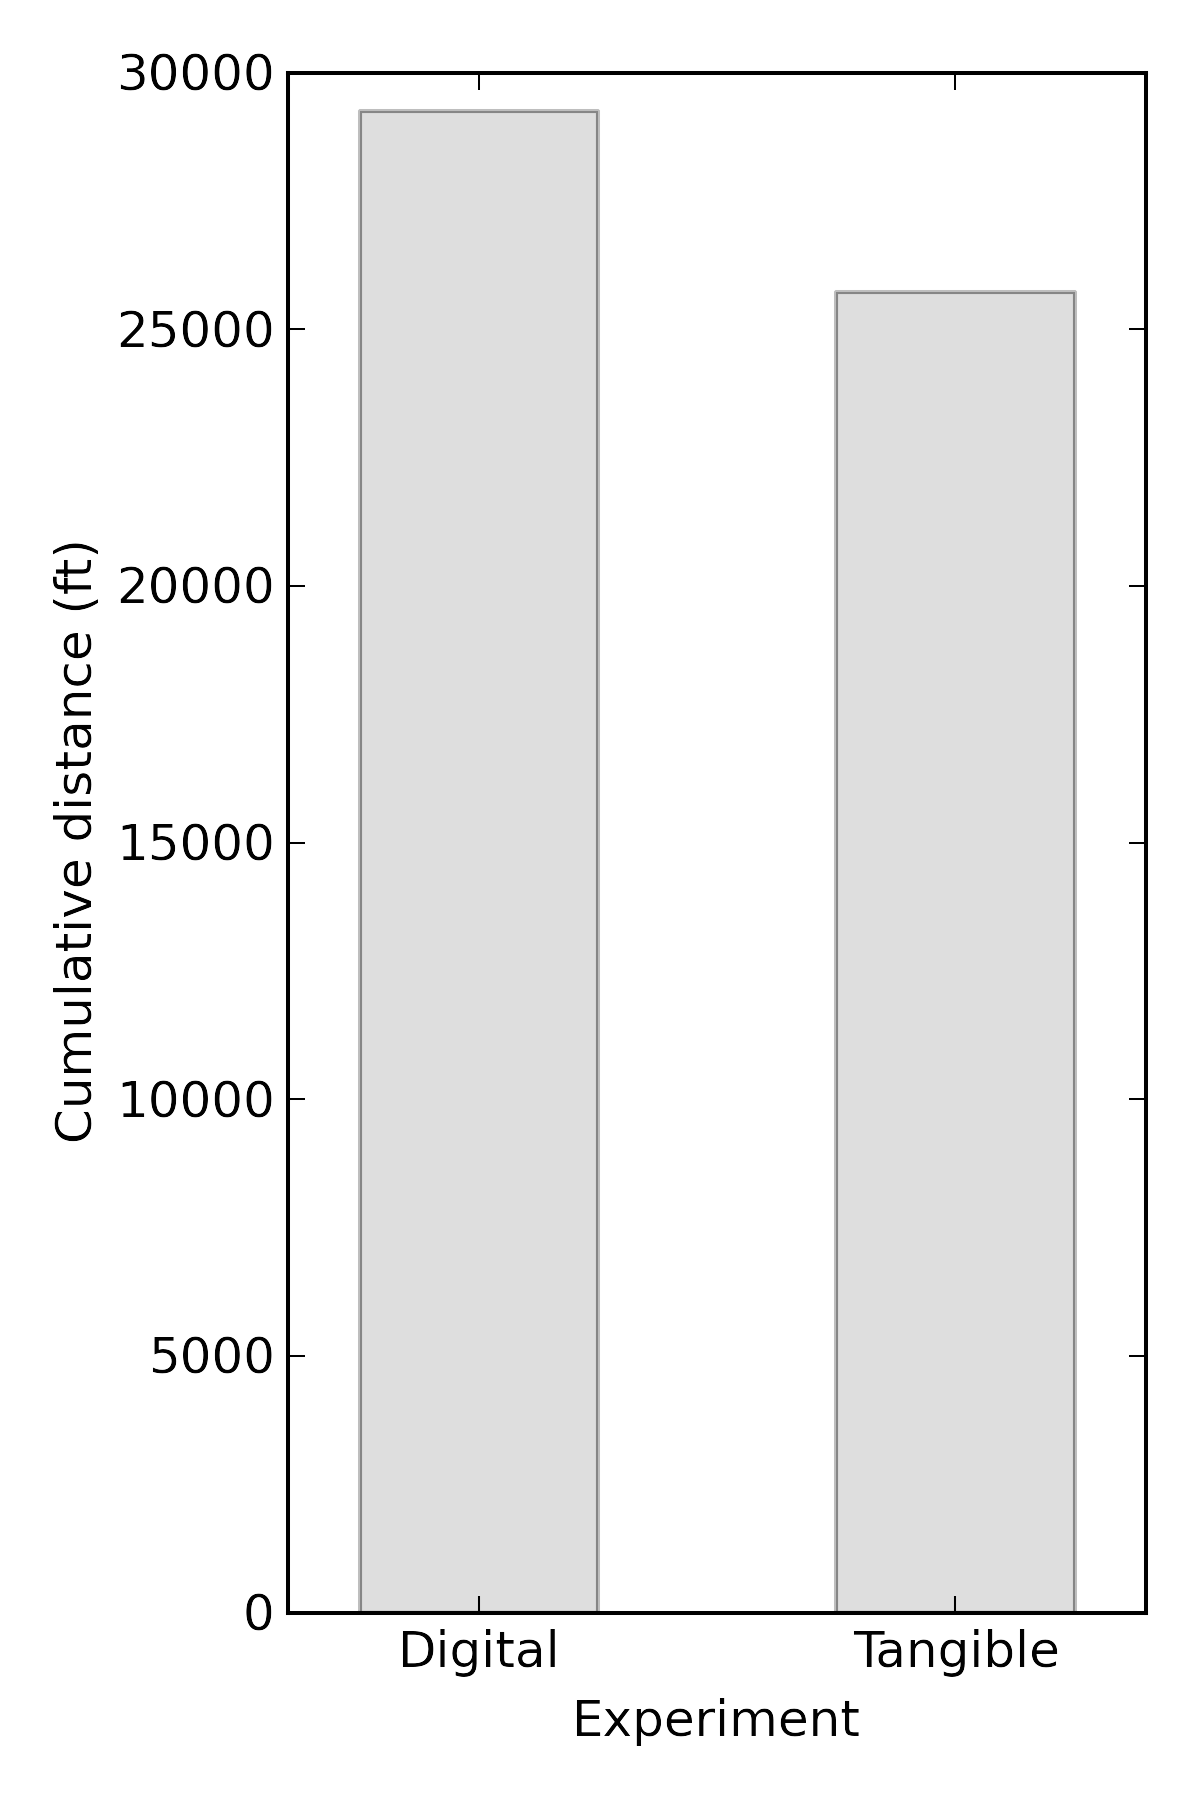
\includegraphics[width=150px]{figures/distance.png}
%\caption{The sum of the minimum distance from cells with high concentrated flow  ($>=$0.05 ft) in the reference to the nearest cell with high concentrated flow for the mean depth of each experiment}
%\label{fig:distance_plot}
%\end{center}
%\end{figure}

% cells with depressions plot
\begin{figure}[ht!]
\begin{center}
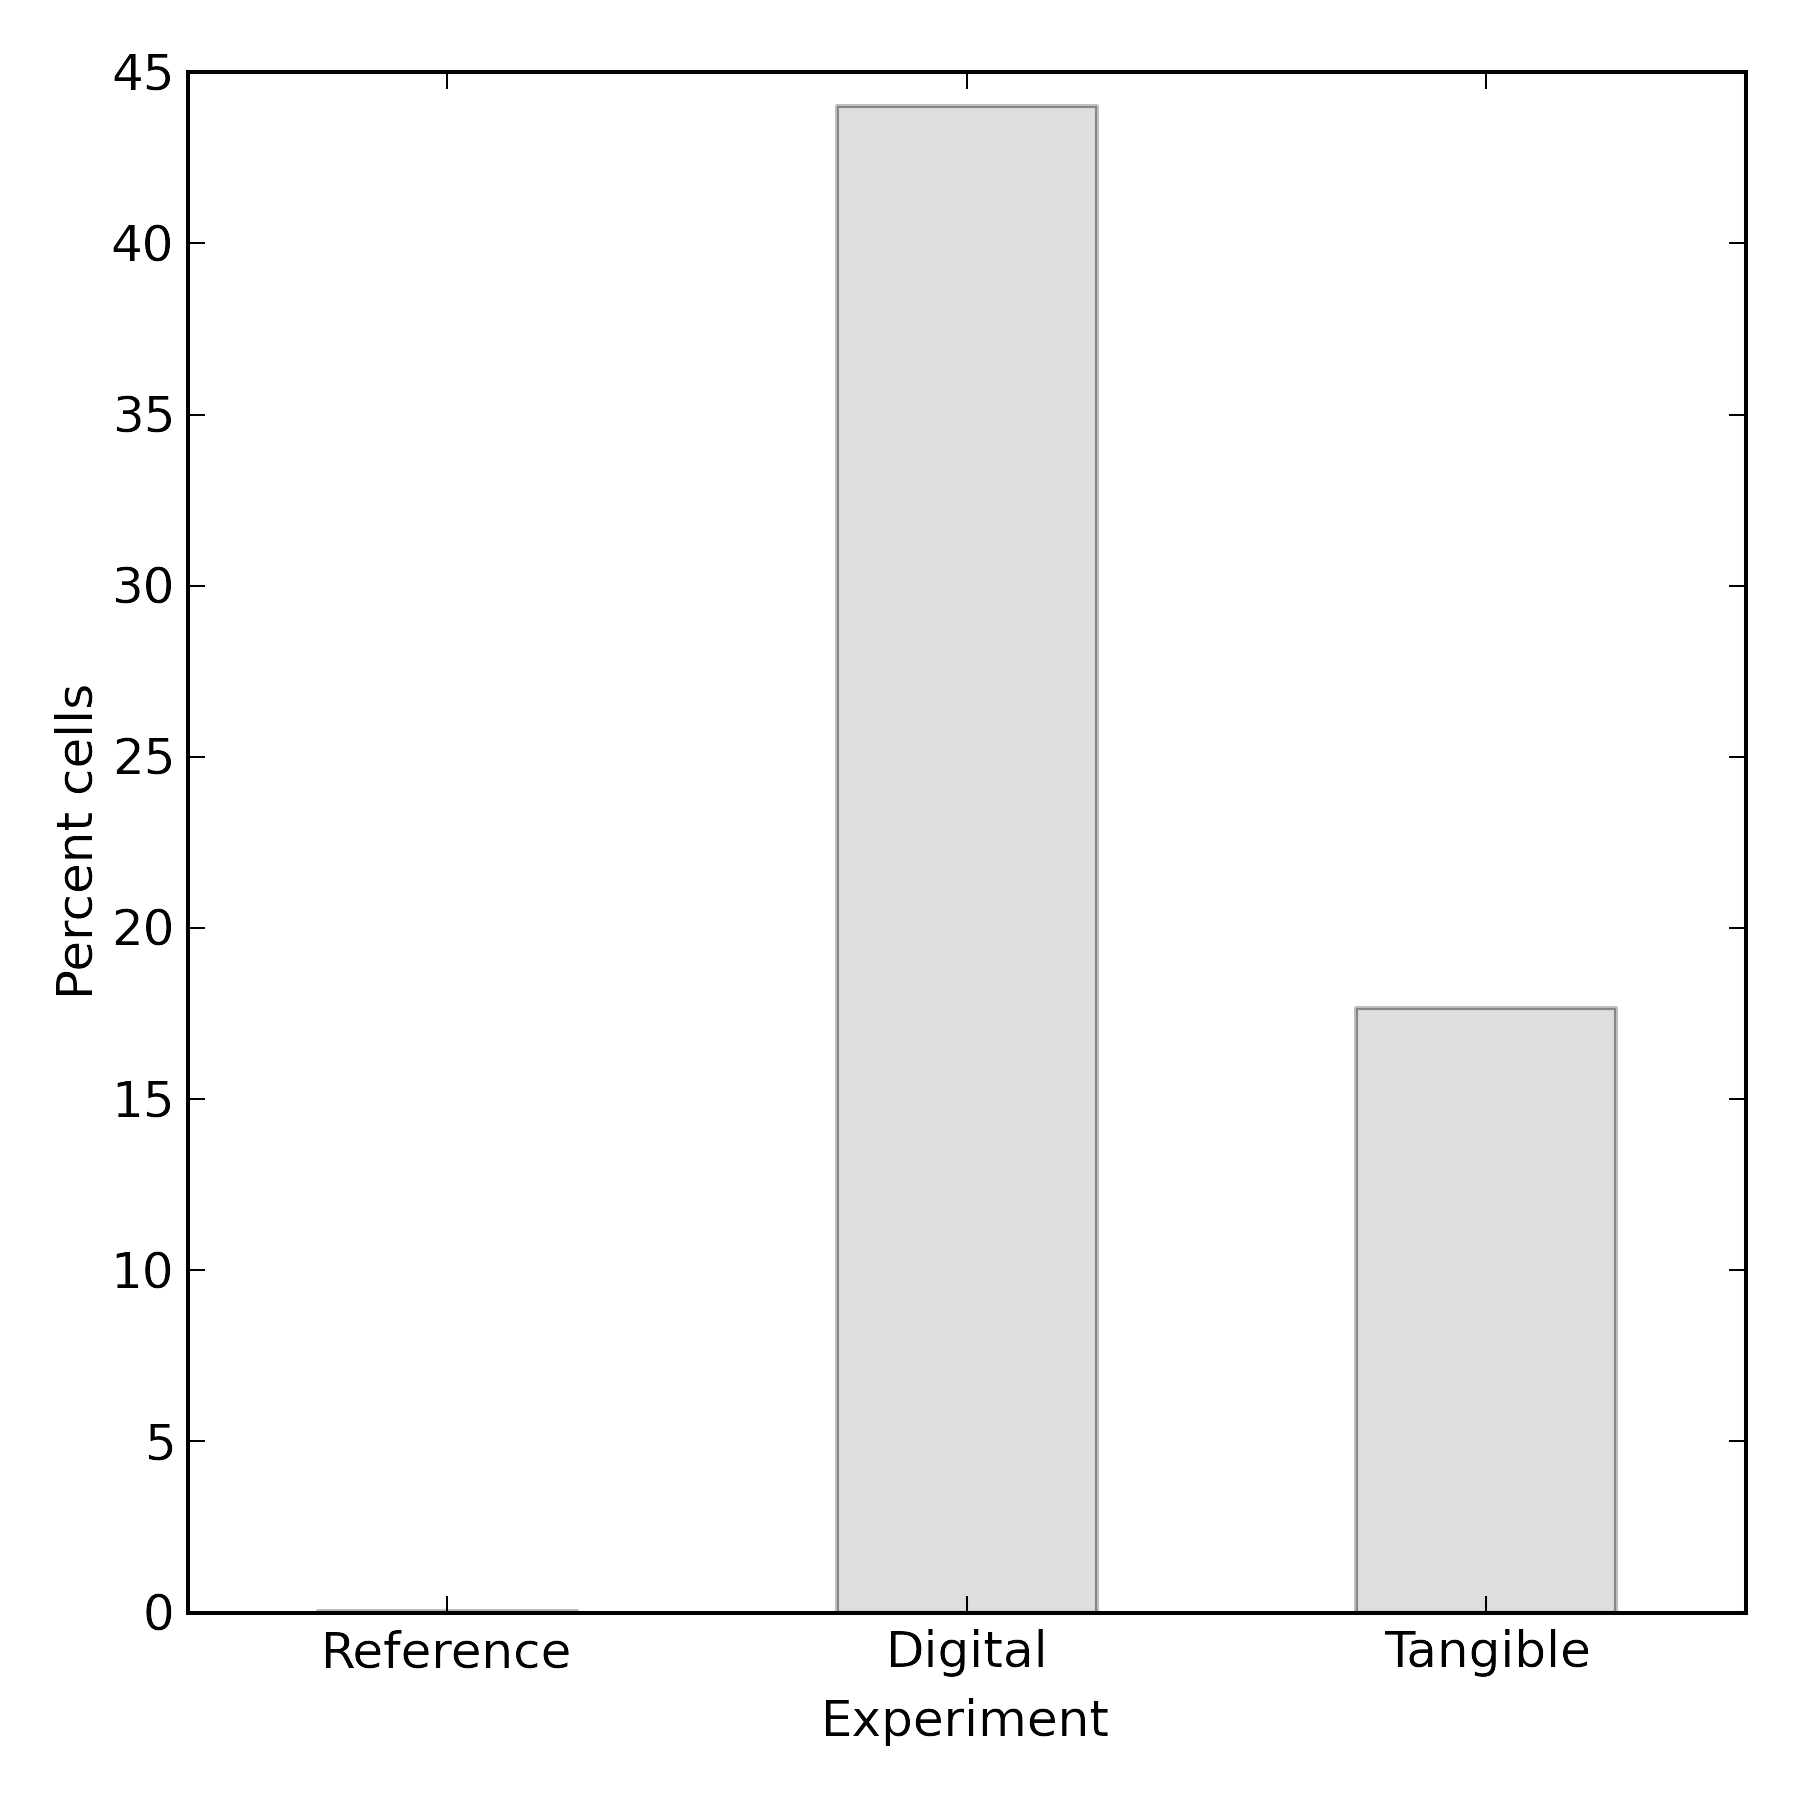
\includegraphics[width=225px]{figures/depression_cells.png}
\caption{Percentage of cells with depressions in (a) the reference landscape, (b) the composite of digitally modeled landscapes, (c) and the composite of tangibly modeled landscapes}
\label{fig:depression_plot}
\end{center}
\end{figure}

% concentrated flow
The models sculpted with Tangible Landscape 
had more concentrated flow in stream channels
with higher 
mean, maximum, and 
summed water depths
(see Table~\ref{table:water_depth}).
%
% concentrated in stream channels
Fig.~\ref{fig:mean_depth}
shows that water flow in the \nth{2} exercise was
spatially concentrated 
in the upper stream channel, 
the lower stream channel, 
and the nascent swale to the right.

% water flow fitting
Furthermore the water flow across models sculpted with Tangible Landscape fit the reference more closely.
Fig.~\ref{fig:mean_diff} and the details in Fig.~\ref{fig:detail_diff} 
show that water flow in the \nth{1} exercise was more spatially diffuse and dispersed, 
whereas water flow in the \nth{2} exercise was a better fit. %fit the reference flow better.
%
Fig.~\ref{fig:distance_1}~-~\ref{fig:distance_2} 
%compare the spatial configuration of concentrated flow to 
show how well the flow of the digitally and tangibly sculpted models fit the reference flow. 
%
The digitally sculpted models tended to loosely fit the upper stream with fewer, more dispersed clusters of concentrated flow at further distances from the reference on average. They also tended to have very few clusters at considerable distance from the swale on the right and small, dispersed clusters that tightly fit the lower stream. 
%
The tangibly sculpted models, however, tended to more densely, tightly fit the upper stream and the swale on the right. 
The tangibly sculpted models tended to miss or misplace the lower stream channel (siting it too far southeast). 
The near-real time water flow analytic was not very useful for modeling the lower stream segment because there was not enough contributing area on the model to generate much concentrated flow. 
Water flow over the sculpted models was only computed over the model, 
whereas the reference water flow was computed over the entire watershed. 
%
Overall the tangibly sculpted models fit the reference flow 8.32\% better than the digitally sculpted models (see Table~\ref{table:distance}).

% depressions
The digitally sculpted models had higher max and summed 
water depth in depressions (see Table~\ref{table:water_depth}).
%
Furthermore the depressions covered 26.34\% more area of the digitally sculpted models than the tangibly sculpted models (see Table~\ref{table:cells}, Fig.~\ref{fig:depression_plot}, and Fig.~\ref{fig:max_depressions}).
%
The presence of large depressions on the central ridge in the \nth{1} exercise reveals 
concave topographic morphology where there should be convex morphology.
%
The pervasive presence of depressions in the stream channels in both exercises 
reveals disrupted flows with broken continuity where water should be flowing. 

\section{Discussion}\label{sec:discussion}
%
The modeling results show that participants tended not to clearly understand how 
topography directs water flow, but began to learn about the importance of curvature and continuity with the aid of the tangible interface. 

% digital results
When digitally sculpting 
participants typically focused on making the streams lower than the surrounding topography, 
but not on draining water into the streams or 
directing a continuous flow downstream.
%
In the \nth{1} exercise participants made low points approximately where the streams should be,
but tended not to grade smooth slopes with appropriate curvature. 
%
The participants use of concave rather than convex morphology on the central ridge reveals that some did not understand how topographic curvature controls water flow.
%
The extensive depressions distributed widely across the terrain
demonstrate that participants tended not understand the importance of topographic curvature and continuity for water flow. 

% tangible results
With the tangible interface they typically focused on directing water into streams,
but did not tend focus on directing a continuous flow downstream.
%
In the \nth{2} exercise participants tended to grade 
smoother slopes with fewer depressions whose curvature directed water towards channels, concentrating it in streams. They, however, did not tend to grade the channels to continuously slope downstream. 
%
While participants performance improved substantially in the \nth{2} exercise, 
the pervasive presence of depressions in the stream channels
in both exercises demonstrates that participants did not fully understand the morphology of streams by the end of the experiment. 

% managing the cognitive load
We observed participants using an iterative modeling process with the tangible interface -- 
they 
\begin{enumerate*}[label=\alph*),font=\itshape]
\item sculpted, 
\item studied the updated water flow simulation, 
\item critiqued the form of their model, 
\item and continued to sculpt
\end{enumerate*}.
%
The substantial improvement in participants' performance in the \nth{2} exercise
shows that they successfully integrated the tangible interface's water flow analytic 
into their modeling process. 
%
To improve their performance they must have been able to successfully manage 
the added cognitive load of the analytical feedback. 
%
The tangibility of the interface may have let them offload some of the cognitive work of sensing and shaping 3D form onto their bodies so that they could focus on water flow. 

% emotions
While their performance did improve in the \nth{2} exercise, it may still have been adversely affected by emotions like frustration. 
%
If the cognitive load of simultaneously modeling 3D form and water flow became too great
-- if participants were unable to fluidly connect cause (topographic form) and effect (flow) --
they might become frustrated and demotivated. 
%
Future research should investigate the role of affect, motivation, and metacognition in tangible interaction.

% more analytics
More analytics may enhance participants understanding of water flow and stream morphology. 
%
Identifying and computing the depth of depressions highlighted the role of topographic curvature and continuity in water flow. 
%
While topographic parameters such as curvature and slope would highlight important aspects of the morphology, 
an additional step of reasoning and imagination is required to link these parameters to water flow. 
%
The ponding of water in depressions directly links topographic controls and water flow 
and thus should be a more intuitive analytic. 
%
We propose combining shallow overland water flow with ponding in depressions
as an analytic to help users understand how water flows. 

\section{Conclusion}\label{sec:conclusion}
%
Tangible Landscape's water flow analytic enabled an iterative cycle of form-finding and critical assessment that helped participants learn how form controls process. 
%
Seeing the water flow simulation update in near real-time 
enabled participants to generate hypotheses, test hypotheses, and draw inferences 
about the way that water flows over topography. 
%
As one participant said, `seeing the flow takes away the mystery of topography.' 
%
Physically manifesting topographic data enables users to cognitively grasp the terrain. 
Coupling the tangible topography with the simulated flow of water 
lets users understand the simulation with their body. 
%-- partially embodying cognition about water flow. 

\begin{figure*}
\begin{center}
\subfigure[]{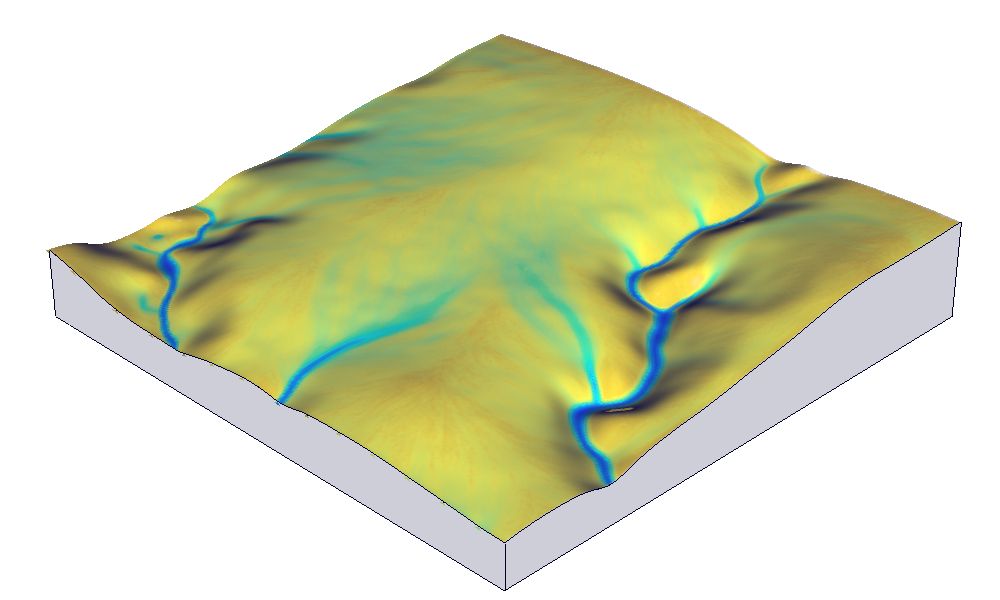
\includegraphics[width=0.3\textwidth]{figures/depth.png}}
\subfigure[]{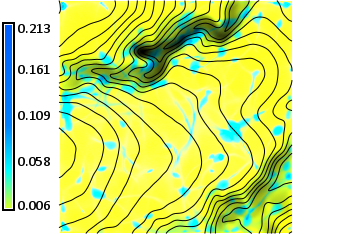
\includegraphics[width=0.3\textwidth]{figures/mean_depth_1.png}}
\subfigure[]{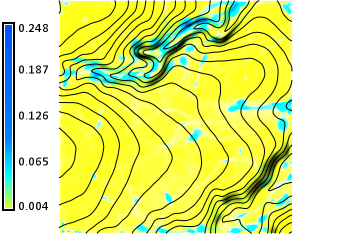
\includegraphics[width=0.3\textwidth]{figures/mean_depth_2.png}}
\caption{(a) The depth of simulated water flow across the reference landscape, (b) the mean depth using digital modeling, (c) and the mean depth using tangible modeling}
\label{fig:mean_depth}
\end{center}
\end{figure*}
%
%\begin{figure*}
%\begin{center}
%\subfigure[]{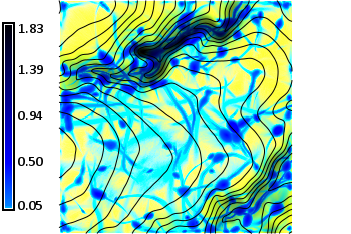
\includegraphics[width=\columnwidth]{figures/max_depth_1.png}}
%\subfigure[]{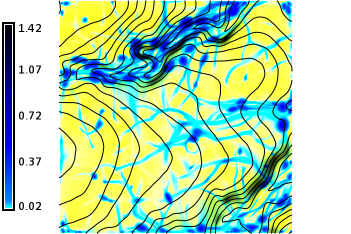
\includegraphics[width=\columnwidth]{figures/max_depth_2.png}}
%\caption{The maximum water depth of all models in (a) the \nth{1} exercise and (b) the \nth{2} exercise}
%\label{fig:max_depth}
%\end{center}
%\end{figure*}
%
%\begin{figure*}
%\begin{center}
%\subfigure[]{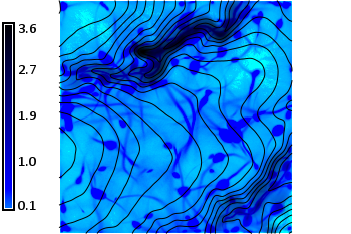
\includegraphics[width=\columnwidth]{figures/sum_depth_1.png}}
%\subfigure[]{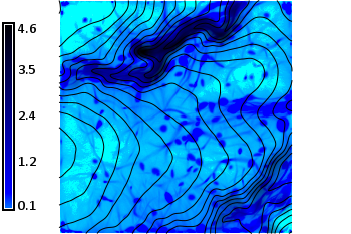
\includegraphics[width=\columnwidth]{figures/sum_depth_2.png}}
%\caption{The sum of the water depths for all models in (a) the \nth{1} exercise and (b) the \nth{2} exercise}
%\label{fig:sum_depth}
%\end{center}
%\end{figure*}
%
\begin{figure*}
\begin{center}
\subfigure[]{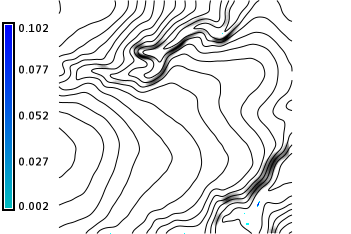
\includegraphics[width=0.3\textwidth]{figures/depressions.png}}
\subfigure[]{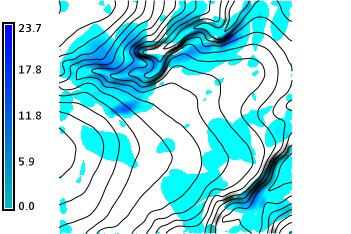
\includegraphics[width=0.3\textwidth]{figures/max_depressions_1.png}}
\subfigure[]{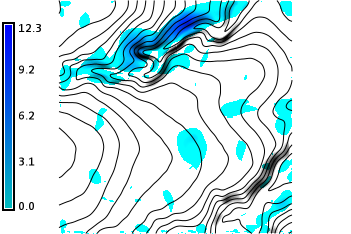
\includegraphics[width=0.3\textwidth]{figures/max_depressions_2.png}}
\caption{(a) The depth of depression in the reference landscape, (b) the maximum depth of depressions using digital modeling, (c) and the maximum depth of depressions using tangible modeling}
\label{fig:max_depressions}
\end{center}
\end{figure*}
%
%\begin{figure*}
%\begin{center}
%\subfigure[]{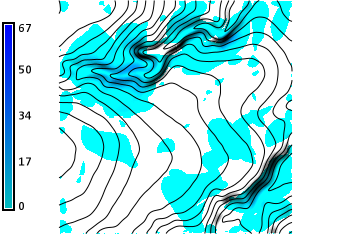
\includegraphics[width=\columnwidth]{figures/sum_depressions_1.png}}
%\subfigure[]{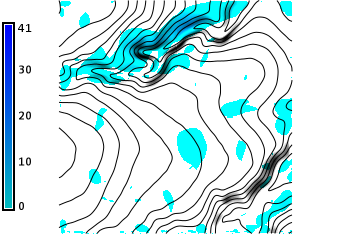
\includegraphics[width=\columnwidth]{figures/sum_depressions_2.png}}
%\caption{The sum of the depth of depressions for all models in (a) the \nth{1} exercise and (b) the \nth{2} exercise}
%\label{fig:sum_depressions}
%\end{center}
%\end{figure*}
%
\begin{figure*}
\begin{center}
\subfigure[]{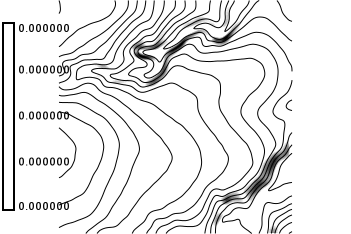
\includegraphics[width=0.3\textwidth]{figures/diff.png}}
\subfigure[]{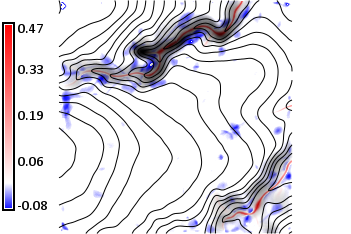
\includegraphics[width=0.3\textwidth]{figures/mean_diff_1.png}}
\subfigure[]{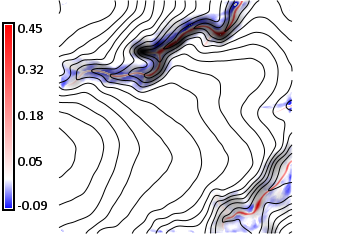
\includegraphics[width=0.3\textwidth]{figures/mean_diff_2.png}}
\caption{(a) The difference of the reference landscape, (b) the mean of digitally sculpted models, (c) and the mean of tangibly sculpted models \textit{from the reference landscape}}
\label{fig:mean_diff}
\end{center}
\end{figure*}
%
\begin{figure*}
\begin{center}
\subfigure[]{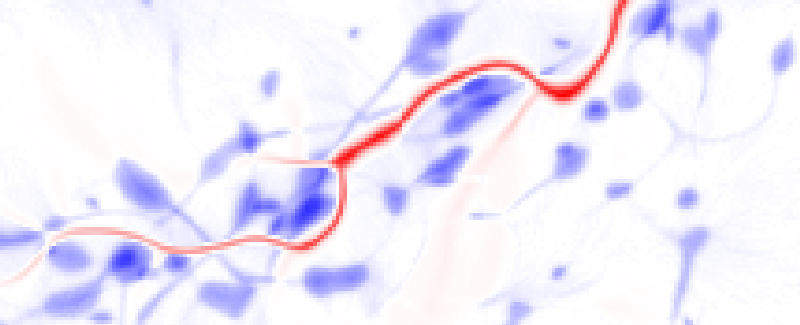
\includegraphics[width=\columnwidth]{figures/detail_diff_1.png}}\hspace{1em}%
\subfigure[]{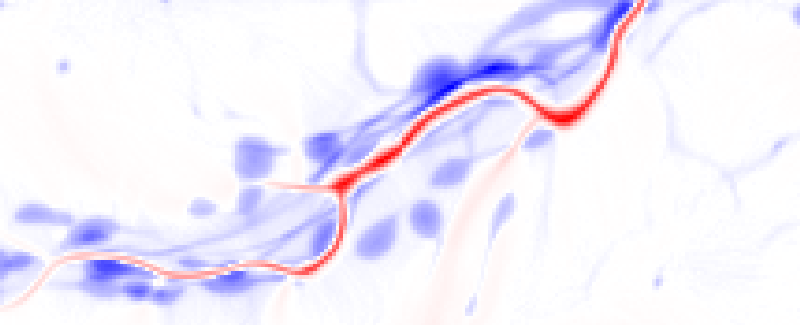
\includegraphics[width=\columnwidth]{figures/detail_diff_2.png}}
\caption{Detail of the difference of (a) the mean of digitally sculpted models and (b) the mean of tangibly sculpted models \textit{from the reference landscape}}
\label{fig:detail_diff}
\end{center}
\end{figure*}
%
%\begin{figure*}
%\begin{center}
%\subfigure[]{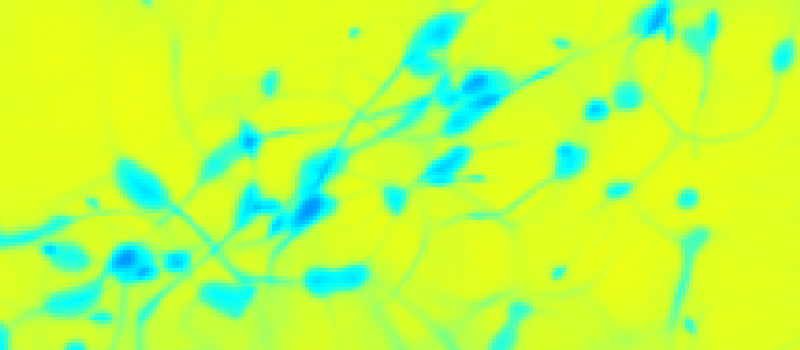
\includegraphics[width=\columnwidth]{figures/mean_depth_detail_1.png}}\hspace{1em}
%\subfigure[]{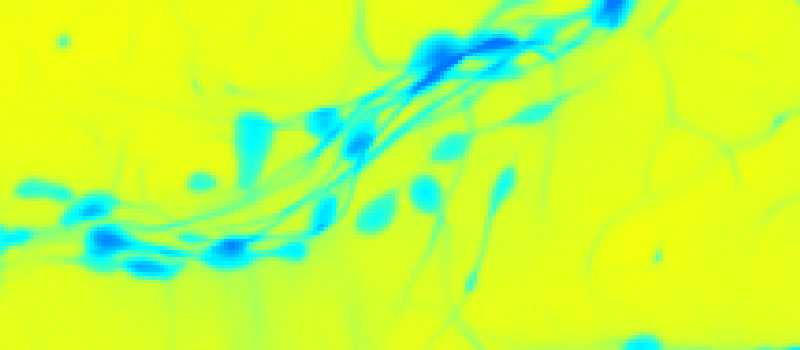
\includegraphics[width=\columnwidth]{figures/mean_depth_detail_2.png}}
%\caption{Detail of the mean depth of (a) digitally sculpted models and (b) tangibly sculpted models}
%\label{fig:detail_diff}
%\end{center}
%\end{figure*}
%
%\begin{figure*}
%\begin{center}
%\subfigure[]{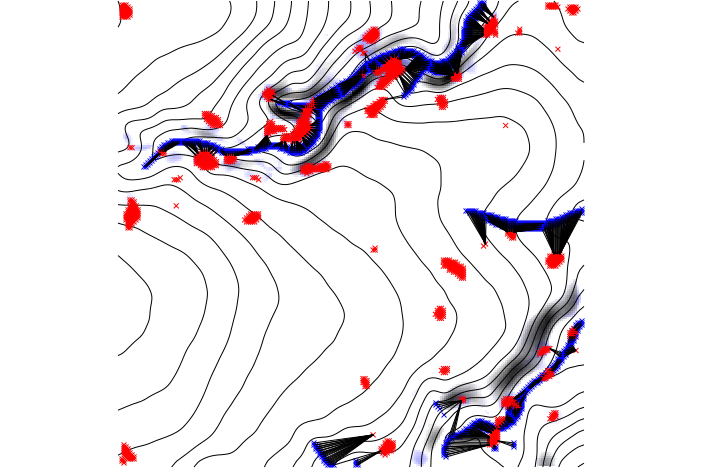
\includegraphics[width=\columnwidth]{figures/concentrated_flow_1.png}}
%\subfigure[]{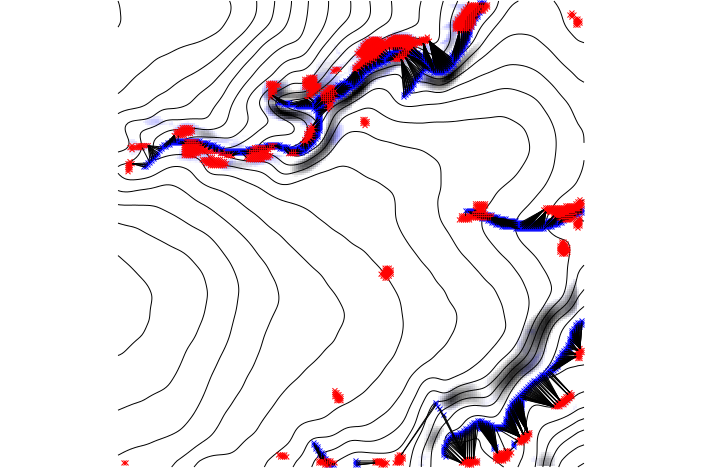
\includegraphics[width=\columnwidth]{figures/concentrated_flow_2.png}}
%\caption{The minimum distance from cells with high concentrated flow  ($>=$0.05 ft) in the reference to the nearest cell with high concentrated flow for the mean depth using (a) digital modeling and (b) tangible modeling}
%\label{fig:mean_depth}
%\end{center}
%\end{figure*}
%
\begin{figure*}
\begin{center}
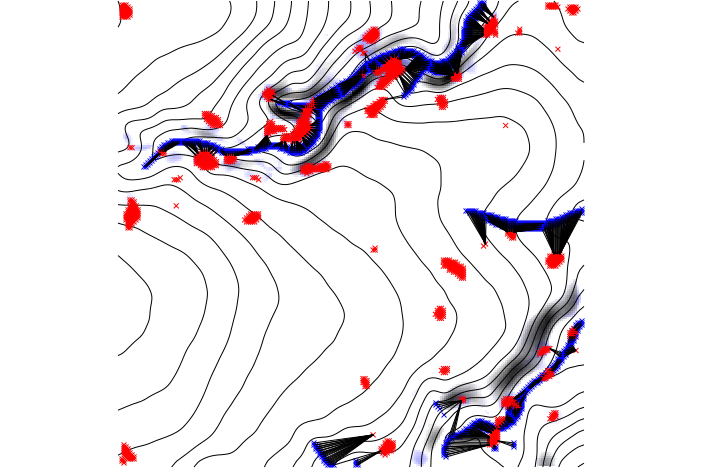
\includegraphics[width=0.9\textwidth]{figures/concentrated_flow_1.png}
\caption{
The lines represent the minimum distance between blue points with high concentrated flow in the reference to red points with high concentrated flow from the mean depth of digitally sculpted models.}
\label{fig:distance_1}
\end{center}
\end{figure*}
%
\begin{figure*}
\begin{center}
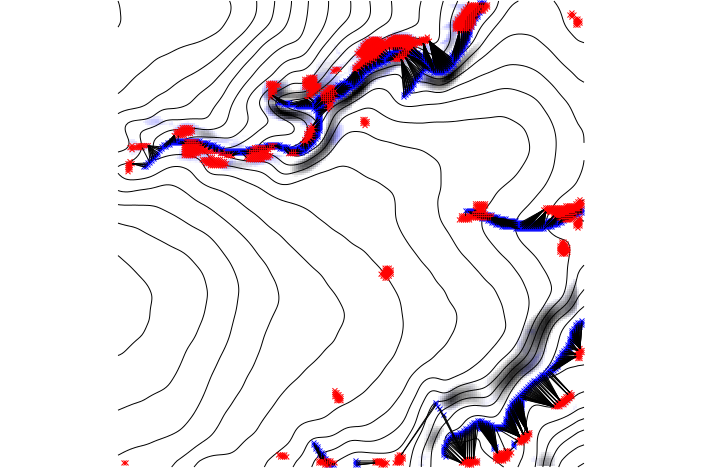
\includegraphics[width=0.9\textwidth]{figures/concentrated_flow_2.png}
\caption{
The lines represent the minimum distance between blue points with high concentrated flow in the reference to red points with high concentrated flow from the mean depth of tangibly sculpted models.}
\label{fig:distance_2}
\end{center}
\end{figure*}

\bibliography{flow} 
\end{document}

\end{document}
